\documentclass[a4paper,11pt]{article}
\input{/home/tof/Documents/Cozy/latex-include/preambule_lua.tex}
\newcommand{\showprof}{show them}  % comment this line if you don't want to see todo environment
\fancyhead[L]{Exercices arbre}
\newdate{madate}{10}{09}{2020}
%\fancyhead[R]{\displaydate{madate}} %\today
%\fancyhead[R]{Seconde - SNT}
%\fancyhead[R]{Première - NSI}
\fancyhead[R]{Terminale - NSI}
\fancyfoot[L]{~\\Christophe Viroulaud}
\AtEndDocument{\label{lastpage}}
\fancyfoot[C]{\textbf{Page \thepage/\pageref{lastpage}}}
\fancyfoot[R]{\includegraphics[width=2cm,align=t]{/home/tof/Documents/Cozy/latex-include/cc.png}}
\usepackage{tikz}

\begin{document}
\begin{Form}
\begin{commentprof}
annexe-exercice-arbre.zip sur site
\end{commentprof}
\begin{center}
\shadowbox{\parbox{14cm}{\centering Télécharger l'annexe \emph{annexe-exercice-arbre.zip} et extraire les fichiers.}}
\end{center}
\begin{exo}
\begin{center}
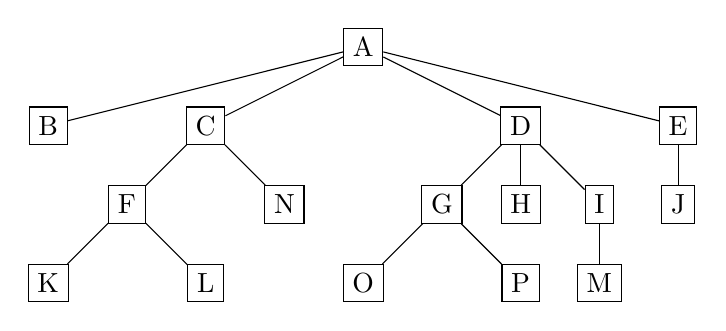
\begin{tikzpicture}
\node[draw] (A) at (0,0) {A};
\node[draw] (B) at (-4,-1) {B};
\node[draw] (C) at (-2,-1) {C};
\node[draw] (D) at (2,-1) {D};
\node[draw] (E) at (4,-1) {E};
\node[draw] (F) at (-3,-2) {F};
\node[draw] (N) at (-1,-2) {N};
\node[draw] (G) at (1,-2) {G};
\node[draw] (H) at (2,-2) {H};
\node[draw] (I) at (3,-2) {I};
\node[draw] (J) at (4,-2) {J};
\node[draw] (K) at (-4,-3) {K};
\node[draw] (L) at (-2,-3) {L};
\node[draw] (M) at (3,-3) {M};
\node[draw] (O) at (0,-3) {O};
\node[draw] (P) at (2,-3) {P};

\draw (A) -- (B);
\draw (A) -- (C);
\draw (A) -- (D);
\draw (A) -- (E);
\draw (C) -- (F);
\draw (C) -- (N);
\draw (D) -- (G);
\draw (D) -- (H);
\draw (D) -- (I);
\draw (E) -- (J);
\draw (F) -- (K);
\draw (F) -- (L);
\draw (G) -- (O);
\draw (G) -- (P);
\draw (I) -- (M);
\end{tikzpicture}
\captionof{figure}{Une structure arborescente}
\label{arbre}
\end{center}
\begin{enumerate}
\item Donner le nom de la racine, le nombre de feuilles, la taille et la profondeur de l'arbre figure \ref{arbre}. On considère qu'un arbre qui n'a qu'une racine est de profondeur 0.
\item Donner un parcours en largeur puis un parcours en profondeur de cette structure arborescente.
\end{enumerate}
\end{exo}
\begin{exo}
Voici deux arborescences de fichiers. Pour chacune d’elles, donner la taille et la hauteur de l’arbre correspondant.
\begin{center}
\centering
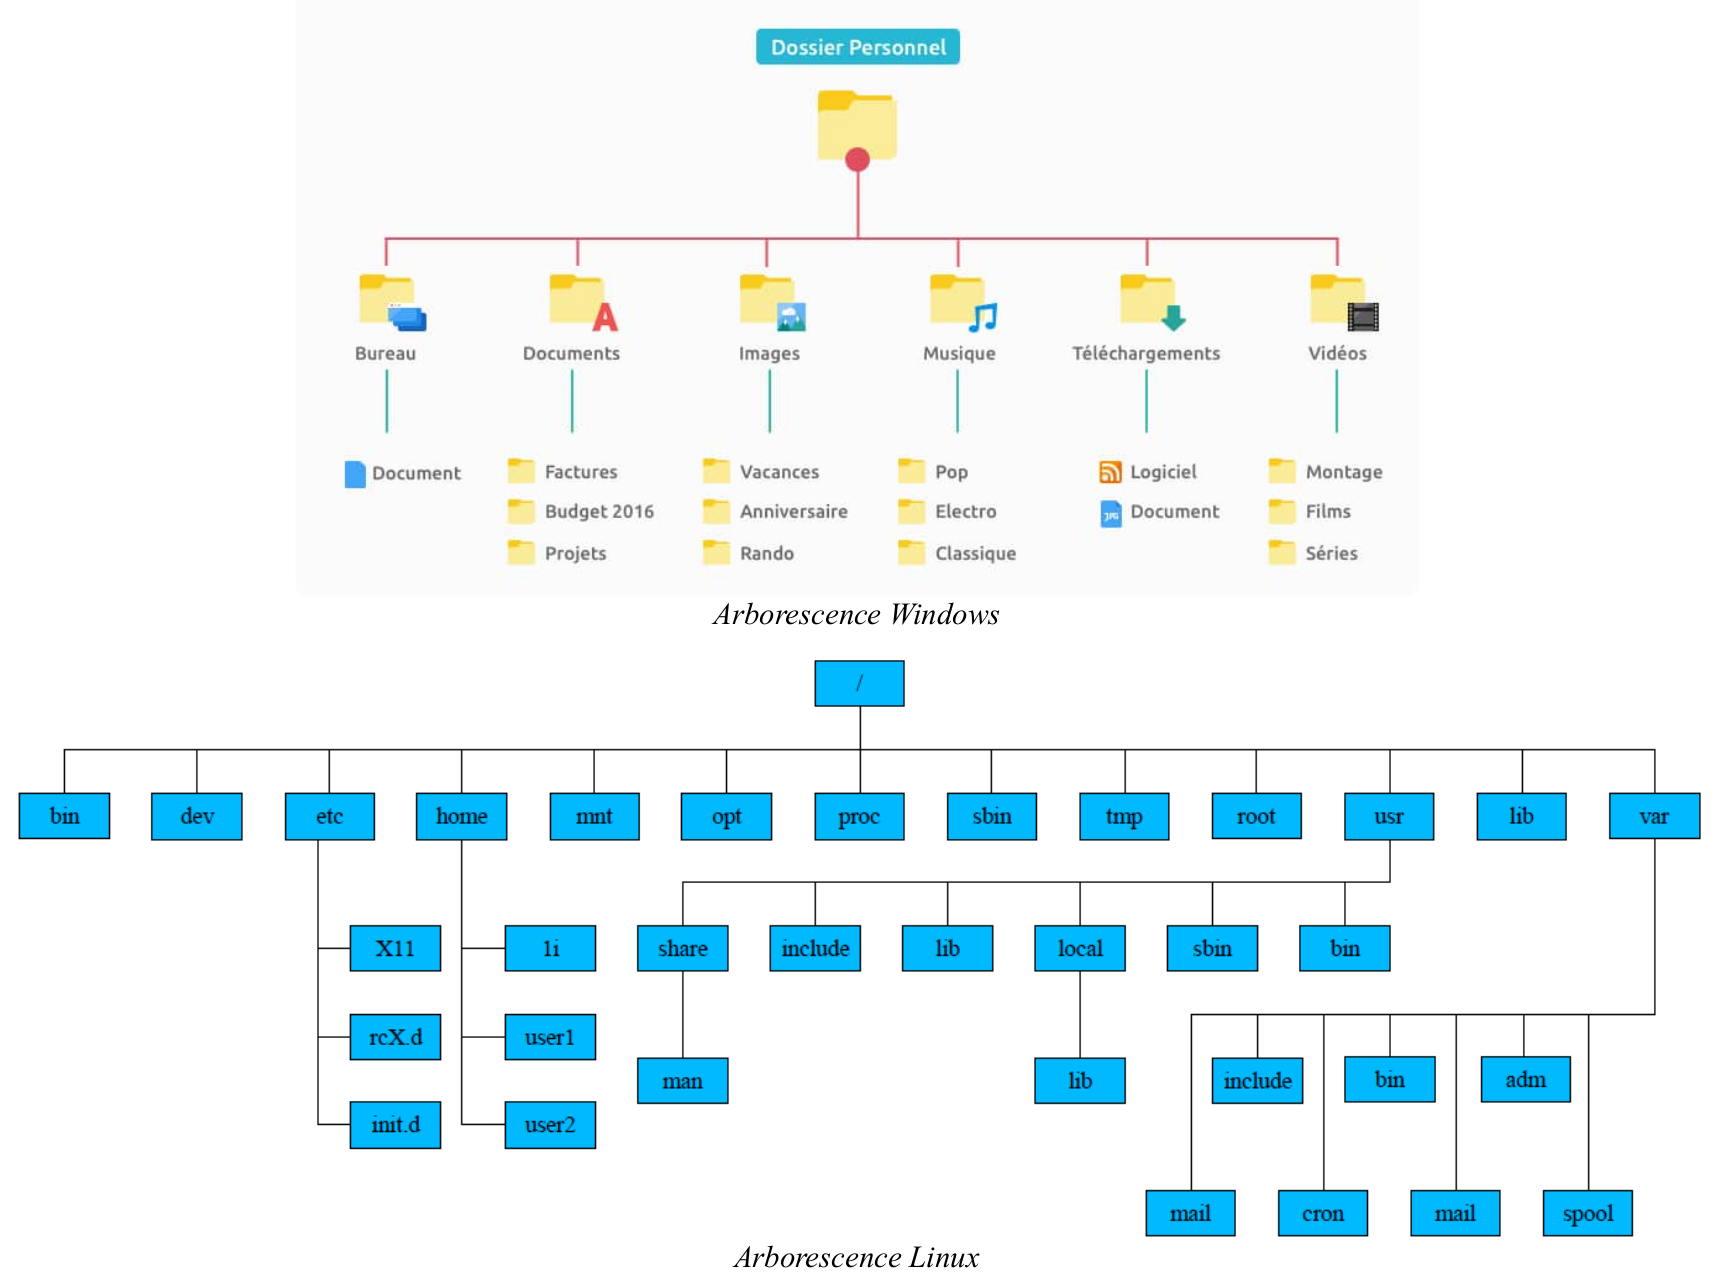
\includegraphics[width=14cm]{ressources/os.png}
\captionof{figure}{Systèmes d'exploitation}
\label{os}
\end{center}


\end{exo}
\begin{exo}
On souhaite réaliser un correcteur orthographique. Pour cela, on a besoin d’un dictionnaire contenant les différents mots
de la langue française. Pour l’instant, on dispose seulement de quelques mots : \emph{arbre, arbitre, arbitrer, binaire, binette, bio, empiler, exact}.\\
On souhaite stocker ces mots par ordre alphabétique dans une liste Python. Chaque nom/adjectif qualificatif sera
présent au singulier et au pluriel, les adjectifs qualificatifs seront également présents au féminin et les verbes seront également conjugués au présent de l’indicatif.
\begin{enumerate}
\item  Quelle sera la taille de cette liste ? En déduire le nombre de tests nécessaires (mot à mot et pas lettre à lettre) pour trouver le mot « exactes » en effectuant une recherche linéaire.
\item Représenter ce dictionnaire rudimentaire sous la forme d’un arbre dans lequel chaque nœud est une lettre. La racine et la fin des mots seront notées avec le symbole *. Combien de tests sont nécessaires pour trouver le mot \emph{« exactes »} ?
\end{enumerate}
\end{exo}
\begin{exo}
Un site web de cuisine stocke chaque recette sous forme d'un fichier \emph{json (JavaScript Object Notation)}.
\begin{enumerate}
\item Ouvrir le fichier \emph{recette-fondant.json} à l'aide d'un éditeur de texte et construire sur papier l'arbre correspondant à la recette. Il faut remarquer qu'il n'y a pas de nœud racine.
\item Ouvrir le fichier \emph{recette.py}. L'arbre a été construit avec la classe \emph{Noeud}.
\item Écrire la fonction \textbf{BFS(arbre: Noeud)$\;\rightarrow\;$list} qui effectue un parcours en largeur de l'arbre et renvoie la liste des valeurs (attribut \emph{valeur)} des nœuds visités.
\item Écrire la fonction \textbf{affiche(arbre: Noeud, decalage: str = "", affichage: str = "")$\;\rightarrow\;$str} qui affiche l'arbre avec un décalage de quatre espaces entre chaque niveau (code \ref{affichage}).
\begin{center}
\begin{lstlisting}[language=Python]
None
    recette
        Fondant au chocolat
    difficulté
        facile
    temps
        préparation
            unite
                min
            valeur
                15
\end{lstlisting}
\captionof{code}{Début d'affichage de l'arbre}
\label{affichage}
\end{center}
\end{enumerate}
\end{exo}


\end{Form}
\end{document}